\section{二次曲面}
在前面两小节中,我们为几何特征很明显的球面、旋转面、柱面、锥面建立了各自的方程.
本小节则对比较简单的二次方程,从方程出发去研究图形的性质.

我们首先给出“二次曲面”的定义:
\begin{definition}
把三元二次方程\(F(x,y,z)=0\)所表示的曲面称为\DefineConcept{二次曲面}(quadratic surface).
%@see: https://mathworld.wolfram.com/QuadraticSurface.html
\end{definition}

我们已经知道,二次方程\begin{equation*}
	\frac{x^2}{a^2}+\frac{y^2}{b^2}-1=0
\end{equation*}表示椭圆柱面,
\begin{equation*}
	\frac{x^2}{a^2}-\frac{y^2}{b^2}+1=0
\end{equation*}表示双曲柱面,
\begin{equation*}
	x^2+2py=0
\end{equation*}表示抛物柱面,
\begin{equation*}
	\frac{x^2}{a^2}+\frac{y^2}{b^2}-\frac{z^2}{c^2}=0
\end{equation*}表示锥面.
现在我们再来研究几个二次方程表示的图形.

\subsection{椭球面}
方程\begin{equation}\label{equation:解析几何.椭球面的一般方程}
	\frac{x^2}{a^2}+\frac{y^2}{b^2}+\frac{z^2}{c^2}=1,
	\quad a,b,c>0
\end{equation}
表示的曲面称为\DefineConcept{椭球面}(ellipsoid).
它有下述性质:
\begin{enumerate}
	\item 对称性.
	因为方程 \labelcref{equation:解析几何.椭球面的一般方程} 中用\(-x\)代\(x\),方程不变,
	于是若点\(P(x,y,z)\)在此椭球面上,
	则点\(P\)关于\(Oyz\)平面的对称点\((-x,y,z)\)也在此椭球面上,
	即此椭球面关于\(Oyz\)平面对称;
	同理,它也关于\(Oxy\)平面、\(Ozx\)平面对称.
	因为方程 \labelcref{equation:解析几何.椭球面的一般方程} 中同时用\(-x\)代\(x\),用\(-y\)代\(y\),方程不变,
	所以此椭球面关于\(z\)轴对称;
	同理,它也关于\(x\)轴、\(y\)轴对称.
	因为方程 \labelcref{equation:解析几何.椭球面的一般方程} 中同时用\(-x\)代\(x\),用\(-y\)代\(y\),用\(-z\)代\(z\),方程不变,
	所以椭球面关于原点对称.

	\item 范围.
	由方程 \labelcref{equation:解析几何.椭球面的一般方程} 立即看出\begin{equation*}
		\abs{x} \leq a, \qquad
		\abs{y} \leq b, \qquad
		\abs{z} \leq c.
	\end{equation*}

	\item 形状.
	此椭球面与\(Oxy\)平面的交线为\begin{equation*}
		\left\{ \begin{array}{l}
			\frac{x^2}{a^2}+\frac{y^2}{b^2}=1, \\
			z = 0.
		\end{array} \right.
	\end{equation*}
	这时在\(Oxy\)平面上的一个椭圆.
	同理可知,此椭球面与\(Oyz\)平面或\(Oxz\)平面的交线也是椭圆.

	用平行于\(Oxy\)平面的平面\(z = h\)截此椭球面得到的交线(称之为\DefineConcept{截口})的方程为\begin{equation*}
		\left\{ \begin{array}{l}
			\frac{x^2}{a^2}+\frac{y^2}{b^2}=1-\frac{h^2}{c^2}, \\
			z = h.
		\end{array} \right.
	\end{equation*}
	当\(\abs{h} < c\)时,截口是椭圆;
	当\(\abs{h} = c\)时,截口是一个点;
	当\(\abs{h} > c\)时,无轨迹.

	\item 等高线.
	把平行于\(Oxy\)平面的截口投影到\(Oxy\)平面上得到的投影线称为\DefineConcept{等高线}.
\end{enumerate}

\begin{example}
试证:椭球面\begin{equation*}
S: \frac{x^2}{a^2} + \frac{y^2}{b^2} + \frac{z^2}{c^2} = 1.
\end{equation*}在其上任意一点\(P_0(x_0,y_0,z_0)\)处的切面方程为
\begin{equation}\label{equation:解析几何.椭球面的切平面}
	\frac{x_0 x}{a^2} + \frac{y_0 y}{b^2} + \frac{z_0 z}{c^2} = 1.
\end{equation}
%TODO
\end{example}

\subsection{单叶双曲面}
方程\begin{equation}\label{equation:解析几何.单叶双曲面}
	\frac{x^2}{a^2}+\frac{y^2}{b^2}-\frac{z^2}{c^2}=1,
	\quad a,b,c>0
\end{equation}
表示的曲面称为\DefineConcept{单叶双曲面}(one-sheeted elliptic hyperboloid).
% 下面绘出单叶双曲面的图形:
%@Mathematica: RevolutionPlot3D[{Sec[t], Tan[t]}, {t, -Pi, Pi}, PlotRange -> {-5, 5}]
它具有下述性质:
\begin{enumerate}
	\item 对称性.
	三个做表面都是此图形的对称平面,三根坐标轴都是它的对称轴,原点是它的对称中心.

	\item 范围.
	由方程 \labelcref{equation:解析几何.单叶双曲面} 得\begin{equation*}
		\frac{x^2}{a^2}+\frac{y^2}{b^2}=1+\frac{z^2}{c^2}\geq1,
	\end{equation*}
	所以此曲面的全在柱面\begin{equation*}
		\frac{x^2}{a^2}+\frac{y^2}{b^2}=1
	\end{equation*}的外部或柱面上.

	\item 形状.
	此曲面与\(Oxy\)平面的交线为\begin{equation*}
		\left\{ \begin{array}{l}
			\frac{x^2}{a^2}+\frac{y^2}{b^2}=1, \\
			z = 0.
		\end{array} \right.
	\end{equation*}
	这是一个椭圆,我们称其为此单叶双曲面的\DefineConcept{腰椭圆}.

	此曲面与\(Ozx\)平面、\(Oyz\)平面的交线分别为\begin{equation*}
		\left\{ \begin{array}{l}
			\frac{x^2}{a^2}-\frac{z^2}{c^2}=1, \\
			y = 0,
		\end{array} \right.
		\qquad
		\left\{ \begin{array}{l}
			\frac{y^2}{b^2}-\frac{z^2}{c^2}=1, \\
			x = 0.
		\end{array} \right.
	\end{equation*}
	它们都是双曲线.

	此曲面的平行于\(Oxy\)平面的截口为\begin{equation*}
		\left\{ \begin{array}{l}
			\frac{x^2}{a^2}+\frac{y^2}{b^2}=1+\frac{h^2}{c^2}, \\
			z = h.
		\end{array} \right.
	\end{equation*}
	这是一个椭圆;
	并且当\(\abs{h}\)增大时,截口椭圆的长、短半轴长\begin{equation*}
		a' = a \sqrt{1+\frac{h^2}{c^2}}, \qquad
		b' = b \sqrt{1+\frac{h^2}{c^2}}
	\end{equation*}均增大.

	\item 渐进锥面.
	锥面\begin{equation}
		\frac{x^2}{a^2}+\frac{y^2}{b^2}-\frac{z^2}{c^2}=0
	\end{equation}
	称为此单叶双曲面的\DefineConcept{渐进锥面}.

	用平面\(z=h\)截此锥面,截口为椭圆\begin{equation*}
		\left\{ \begin{array}{l}
			\frac{x^2}{a^2}+\frac{y^2}{b^2}=\frac{h^2}{c^2}, \\
			z = h.
		\end{array} \right.
	\end{equation*}
	这个椭圆的长、短半轴长分别为\begin{equation*}
		a'' = a \frac{\abs{h}}{c}, \qquad
		b'' = b \frac{\abs{h}}{c}.
	\end{equation*}
	因为\begin{equation*}
		a' - a'' = \frac{a}{\sqrt{1+\frac{h^2}{c^2}}+\frac{\abs{h}}{c}},
	\end{equation*}
	所以\(\lim_{\abs{h}\to\infty}(a'-a'')=0\).
	同理,\(\lim_{\abs{h}\to\infty}(b'-b'')=0\).
	这说明,当\(\abs{h}\)无限增大时,单叶双曲面的截口椭圆与它的渐进锥面的截口椭圆任意接近,
	即单叶双曲面与它的渐进锥面无限地任意接近.
\end{enumerate}

\subsection{双叶双曲面}
方程\begin{equation}\label{equation:解析几何.双叶双曲面}
	\frac{x^2}{a^2}+\frac{y^2}{b^2}-\frac{z^2}{c^2}=-1,
	\quad a,b,c>0
\end{equation}
表示的曲面称为\DefineConcept{双叶双曲面}(two-sheeted elliptic hyperboloid).
% 下面绘出双叶双曲面的图形:
%@Mathematica: RevolutionPlot3D[{Tan[t], Sec[t]}, {t, -Pi, Pi}, PlotRange -> {-5, 5}]
它具有下述性质:
\begin{enumerate}
	\item 对称性.
	它关于坐标面、坐标轴、原点均对称.

	\item 范围.
	由方程 \labelcref{equation:解析几何.双叶双曲面} 得\(\abs{z} \geq c\).

	\item 形状.
	此曲面与\(Oxy\)平面无交点.
	它与\(Ozx\)平面、\(Oyz\)平面的交线分别为\begin{equation*}
		\left\{ \begin{array}{l}
			\frac{z^2}{c^2}-\frac{x^2}{a^2}=1, \\
			y = 0,
		\end{array} \right.
		\qquad
		\left\{ \begin{array}{l}
			\frac{z^2}{c^2}-\frac{y^2}{b^2}=1, \\
			x = 0.
		\end{array} \right.
	\end{equation*}
	它们都是双曲线.

	用平面\(z=h\ (\abs{h}\geq c)\)去截此曲面得到的截口为\begin{equation*}
		\left\{ \begin{array}{l}
			\frac{x^2}{a^2}+\frac{y^2}{b^2}=\frac{h^2}{c^2}-1, \\
			z = h.
		\end{array} \right.
	\end{equation*}
	这是一个椭圆或一个点.

	\item 渐进锥面.
	锥面\begin{equation*}
		\frac{x^2}{a^2}+\frac{y^2}{b^2}-\frac{z^2}{c^2}=0
	\end{equation*}也是此双叶双曲面的渐进锥面.
\end{enumerate}

\subsection{椭圆抛物面}
方程\begin{equation}\label{equation:解析几何.椭圆抛物面的一般方程}
	\frac{x^2}{p}+\frac{y^2}{q}=2z,
	\quad p,q>0
\end{equation}
表示的曲面称为\DefineConcept{椭圆抛物面}.
它的图形如\cref{figure:解析几何.椭圆抛物面} 所示.
它具有下述性质:
\begin{enumerate}
	\item 对称性.
	\(Ozx\)平面、\(Oyz\)平面是它的对称平面,
	\(z\)轴是它的对称轴.

	\item 范围.
	由方程 \labelcref{equation:解析几何.椭圆抛物面的一般方程} 得\(z \geq 0\).

	\item 形状.
	它与\(Ozx\)平面、\(Oyz\)平面的交线分别为\begin{equation*}
		\left\{ \begin{array}{l}
			x^2 = 2pz, \\
			y = 0,
		\end{array} \right.
		\qquad
		\left\{ \begin{array}{l}
			y^2 = 2qz, \\
			x = 0.
		\end{array} \right.
	\end{equation*}
	它们都是抛物线.

	用平面\(z = h\ (h\geq0)\)去截此曲面得到的截口为\begin{equation*}
		\left\{ \begin{array}{l}
			\frac{x^2}{p} + \frac{y^2}{q} = 2h, \\
			z = h,
		\end{array} \right.
	\end{equation*}
	它是一个椭圆或一个点.
\end{enumerate}

\begin{figure}[htb]%椭圆抛物面
	\centering
	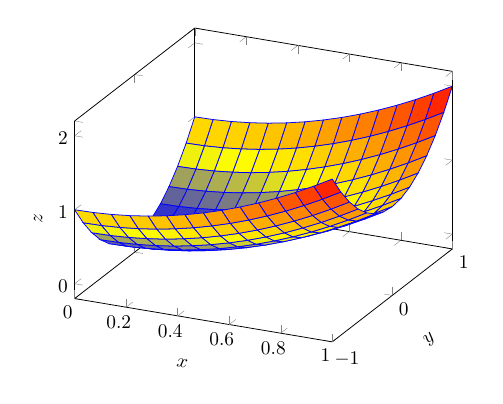
\begin{tikzpicture}[scale=.7]
		\begin{axis}[
			xlabel=$x$,
			ylabel=$y$,
			zlabel=$z$,
			xlabel style={sloped},
			ylabel style={sloped},
		]
			\addplot3[
				surf,
				faceted color=blue,
				samples=15,
				domain=0:1,y domain=-1:1
			]{x^2 + y^2};
		\end{axis}
	\end{tikzpicture}
	\caption{}
	\label{figure:解析几何.椭圆抛物面}
\end{figure}

\subsection{双曲抛物面}
方程\begin{equation}\label{equation:解析几何.双曲抛物面的一般方程}
	\frac{x^2}{p}-\frac{y^2}{q}=2z,
	\quad p,q>0
\end{equation}
表示的曲面称为\DefineConcept{双曲抛物面}或\DefineConcept{马鞍面}.
它的图形如\cref{figure:解析几何.双曲抛物面} 所示.
它具有下述性质:
\begin{enumerate}
	\item 对称性.
	\(Ozx\)平面和\(Oyz\)平面都是双曲抛物面的对称平面,\(z\)轴是它的对称轴.

	\item 形状.
	双曲抛物面与\(Oxy\)平面的交线为\begin{equation*}
		\left\{ \begin{array}{l}
			\frac{x^2}{p} - \frac{y^2}{q} = 0, \\
			z = 0.
		\end{array} \right.
	\end{equation*}
	这时一对经过原点的相交直线.

	双曲抛物面与\(Ozx\)平面、\(Oyz\)平面的交线分别为\begin{equation*}
		\left\{ \begin{array}{l}
			x^2 = 2pz, \\
			y = 0,
		\end{array} \right.
		\qquad
		\left\{ \begin{array}{l}
			y^2 = -2qz, \\
			x = 0;
		\end{array} \right.
	\end{equation*}
	它们都是抛物线.

	用平面\(z=h\ (h\neq0)\)去截此曲面,得到的截口为\begin{equation*}
		\left\{ \begin{array}{l}
			\frac{x^2}{p} - \frac{y^2}{q} = 2h, \\
			z = h.
		\end{array} \right.
	\end{equation*}
	这是一条双曲线;
	当\(h>0\)时,它的实轴平行于\(x\)轴;
	当\(h<0\)时,它的实轴平行于\(y\)轴.

	当平行移动抛物线\begin{equation*}
		\left\{ \begin{array}{l}
			y^2 = -2qz, \\
			x = 0,
		\end{array} \right.
	\end{equation*}
	使得它的顶点沿抛物线\begin{equation*}
		\left\{ \begin{array}{l}
			x^2 = 2pz, \\
			y = 0
		\end{array} \right.
	\end{equation*}移动时,
	便得到马鞍面.
	这是因为,点\(M(x,y,z)\)在此轨迹上的充分必要条件是:
	\(M\)在以抛物线\begin{equation*}
		\left\{ \begin{array}{l}
			x^2 = 2pz, \\
			y = 0
		\end{array} \right.
	\end{equation*}上的一个点\(M_0(x_0,y_0,z_0)\)为顶点,
	且轴平行于\(z\)轴,
	形状、开口与\begin{equation*}
		\left\{ \begin{array}{l}
			y^2 = -2qz, \\
			x = 0
		\end{array} \right.
	\end{equation*}一样的抛物线上,即有\begin{equation*}
		\left\{ \begin{array}{l}
			x_0^2 = 2pz_0, \\
			y_0 = 0, \\
			y^2 = -2q(z-z_0), \\
			x = x_0;
		\end{array} \right.
	\end{equation*}
	消去\(x_0,y_0,z_0\),得到\begin{equation*}
		y^2=-2q\left(z - \frac{x^2}{2p}\right),
	\end{equation*}
	整理得\begin{equation*}
		\frac{x^2}{p} - \frac{y^2}{q} = 2z.
	\end{equation*}
\end{enumerate}

\begin{figure}[htb]%双曲抛物面
	\centering
	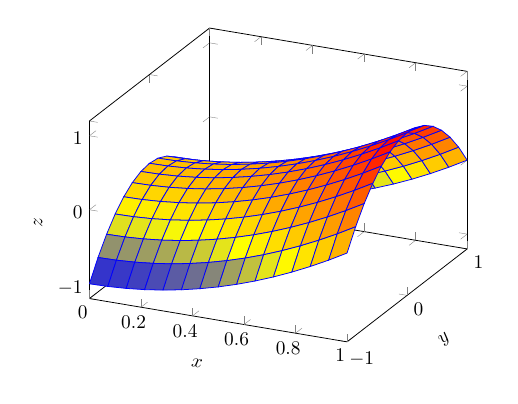
\begin{tikzpicture}[scale=.7]
		\begin{axis}[
			xlabel=$x$,
			ylabel=$y$,
			zlabel=$z$,
			xlabel style={sloped},
			ylabel style={sloped},
		]
			\addplot3[
				surf,
				faceted color=blue,
				samples=15,
				domain=0:1,y domain=-1:1
			]{x^2 - y^2};
		\end{axis}
	\end{tikzpicture}
	\caption{}
	\label{figure:解析几何.双曲抛物面}
\end{figure}

\subsection{二次曲面的种类}\label{section:解析几何.二次曲面的种类}
到目前为止,我们学过的二次曲面有以下17种:
\begin{enumerate}[label={\chinese*.}]
	\item 椭球面
	\begin{enumerate}[label={\arabic*.}]
		\item 椭球面:\begin{equation*}
			\frac{x^2}{a^2}+\frac{y^2}{b^2}+\frac{z^2}{c^2}=1;
		\end{equation*}

		\item 虚椭球面:\begin{equation*}
			\frac{x^2}{a^2}+\frac{y^2}{b^2}+\frac{z^2}{c^2}=-1;
		\end{equation*}

		\item 点:\begin{equation*}
			\frac{x^2}{a^2}+\frac{y^2}{b^2}+\frac{z^2}{c^2}=0;
		\end{equation*}
	\end{enumerate}

	\item 双曲面
	\begin{enumerate}[label={\arabic*.}]
		\setcounter{enumii}{3}
		\item 单叶双曲面:\begin{equation*}
			\frac{x^2}{a^2}+\frac{y^2}{b^2}-\frac{z^2}{c^2}=1;
		\end{equation*}

		\item 双叶双曲面:\begin{equation*}
			\frac{x^2}{a^2}+\frac{y^2}{b^2}-\frac{z^2}{c^2}=-1;
		\end{equation*}
	\end{enumerate}

	\item 抛物面
	\begin{enumerate}[label={\arabic*.}]
		\setcounter{enumii}{5}
		\item 椭圆抛物面:\begin{equation*}
			\frac{x^2}{p}+\frac{y^2}{q}=2z;
		\end{equation*}

		\item 双曲抛物面:\begin{equation*}
			\frac{x^2}{p}-\frac{y^2}{q}=2z;
		\end{equation*}
	\end{enumerate}

	\item 二次锥面
	\begin{enumerate}[label={\arabic*.}]
		\setcounter{enumii}{7}
		\item 二次锥面:\begin{equation*}
			\frac{x^2}{a^2}+\frac{y^2}{b^2}-\frac{z^2}{c^2}=0;
		\end{equation*}
	\end{enumerate}

	\item 二次柱面
	\begin{enumerate}[label={\arabic*.}]
		\setcounter{enumii}{8}
		\item 椭圆柱面:\begin{equation*}
			\frac{x^2}{a^2}+\frac{y^2}{b^2}=1;
		\end{equation*}

		\item 虚椭圆柱面:\begin{equation*}
			\frac{x^2}{a^2}+\frac{y^2}{b^2}=-1;
		\end{equation*}

		\item 直线:\begin{equation*}
			\frac{x^2}{a^2}+\frac{y^2}{b^2}=0;
		\end{equation*}

		\item 双曲柱面:\begin{equation*}
			\frac{x^2}{a^2}-\frac{y^2}{b^2}=1;
		\end{equation*}

		\item 一对相交平面:\begin{equation*}
			\frac{x^2}{a^2}-\frac{y^2}{b^2}=0;
		\end{equation*}

		\item 抛物柱面:\begin{equation*}
			x^2=2py;
		\end{equation*}

		\item 一对平行平面:\begin{equation*}
			x^2=a^2;
		\end{equation*}

		\item 一对虚平行平面:\begin{equation*}
			x^2=-a^2;
		\end{equation*}

		\item 一对重合平面:\begin{equation*}
			x^2=0.
		\end{equation*}
	\end{enumerate}
\end{enumerate}
我们可以证明二次曲面只有这17种.

不过有的地方也只考虑以下9种曲面是二次曲面:
\begin{enumerate}
	\item 椭圆锥面
	\item 椭球面
	\item 单叶双曲面
	\item 双叶双曲面
	\item 椭圆抛物面
	\item 双曲抛物面
	\item 椭圆柱面
	\item 双曲柱面
	\item 抛物柱面
\end{enumerate}
